\chapter{Erstellung des Projekts}
Schon bei der Erstellung des Projekts müssen einige Fragen geklärt werden. Als erstes sollte man
sich wohl fragen, mit welcher CLI man das Projekt erstellen möchte.

Mit CLI (für engl. command-line-interface) ist in unserem Kontext eine Sammlung von Befehlen
gemeint, die in der Kommandozeile eines PCs ausgeführt werden können. Beispiele für Kommandozeilen-
Emulatoren:

\begin{itemize}
  \item Windows Powershell
  \item Windows Cmd
  \item MacOS zsh
  \item Git Bash
  \item Gnome Shell
\end{itemize}

\newpage
\section{React Native CLI}
\textbf{Wichtig}: In der Installationsanleitung auf der Webseite von React Native kann man sein
aktuelles Betriebssystem und Zielplattform auswählen. Apple erlaubt nicht die Entwicklung von Apps
auf anderen Betriebssystemen als MacOS selbst, d.h. die Entwicklung der iOS-App ist auf Windows 11,
meinem Betriebssystem, nicht möglich. Ich hatte während der Entwicklung nie Zugriff auf einen PC mit
MacOS, daher wurde die gesamte App ausschließlich für Android entwickelt. Doch sollten wir jemals
diese App wirklich veröffentlichen wollen, so wird das Umschreiben keinen großen Aufwand darstellen,
da wir immer darauf geachtet haben, nur Bibliotheken zu verwenden, die auch für iOS kompatibel sind.

\subsection{Abhängigkeiten und Erstellung des Projekts}
Für die Verwendung der React-Native-CLI werden einige andere Softwarepakete benötigt, darunter --
natürlich -- \nameref{nodejs}, mindestens Version 12. Außerdem wird benötigt:

\begin{itemize}
  \item Java SE Development Kit (mind. Version 11)
  \item Android Studio
  \begin{itemize}
    \item Android SDK 11 (R)
    \item Android SDK Platform: API Level 30
    \item Android Virtual Device: Google Pixel 2 mit Android 11
  \end{itemize}
\end{itemize}

Sobald alle Abhängigkeiten installiert wurden, führt man folgenden Befehl aus, um ein neues React
Native Projekt zu erstellen:

\begin{lstlisting}
C:\example> npx react-native init reactNativeInit
\end{lstlisting}

NPX ist ein Befehl, der seit Version 5.2.0 in NPM enthalten ist. Er ist speziell bei CLIs hilfreich,
denn anstatt das Paket react-native auf dem PC zu installieren und dann aufzurufen, wird mit dem
Befehl automatisch die neueste Version der CLI von einem Server abgefragt und ausgeführt. So kann
man sicherstellen, dass niemals eine veraltete Version der CLI verwendet wird.

\subsubsection{Metro}
\label{metrobundler}
Beim Start der App wird als erstes der Metro Bundler initialisiert. Er besteht aus einem Server,
welcher den geschriebenen Code mittels Babel kompiliert und anschließend an die App schickt. Dadurch
verhindert man, jedes mal die App neu auf das Gerät installieren zu müssen, um eine kleine Änderung
im Text sehen zu können. Beim Einbinden von neuen JavaScript-Bibliotheken muss allerdings der
Bundler neu gestartet werden, um diese verwenden zu können.

Um den Server zu starten gibt man folgenden Befehl ein:

\begin{lstlisting}
C:\example\reactNativeInit> npm start
\end{lstlisting}

Dies ist die Kurzschreibweise für den Befehl npm run start. Start ist nämlich ein Skript in der
Datei package.json.

\begin{figure}[H]
  \begin{center}
    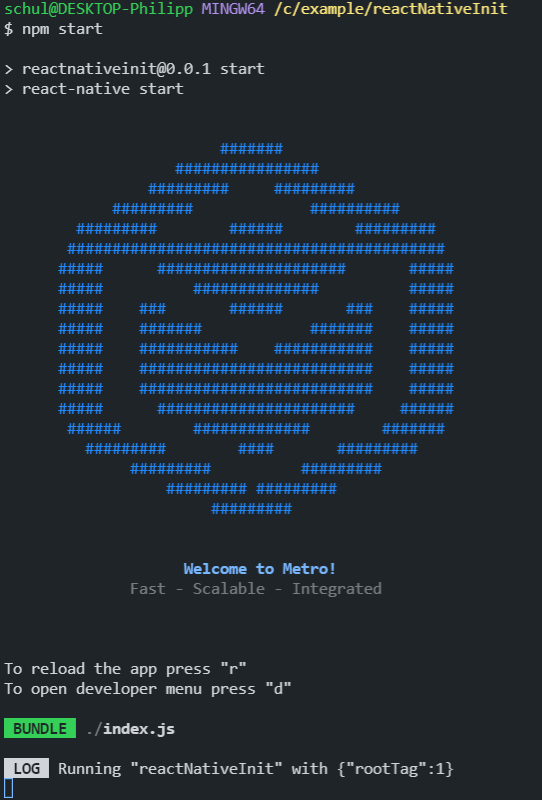
\includegraphics[width=0.5\textwidth]{Theorie/ReactNative/MetroBundler.png}
    \caption{Der Metro-Server in Aktion}
  \end{center}
\end{figure}

Als nächstes öffnet man den Ordner root/android in Android Studio. Man hat nun zwei Möglichkeiten,
die App auszuführen:

\begin{enumerate}
  \item Mit einem virtuellen Android Gerät (Android Virtual Device AVD):\\
Dazu öffnet man in Android Studio den AVD-Manager und erstellt einen neuen Emulator mit einer
Android Version von 11. Danach startet man den Emulator und führt folgenden Befehl aus:

\begin{lstlisting}
C:\example\reactNativeInit> npm run android
\end{lstlisting}

Die App wird auf dem Emulator installiert und ausgeführt.

\begin{figure}[H]
  \begin{center}
    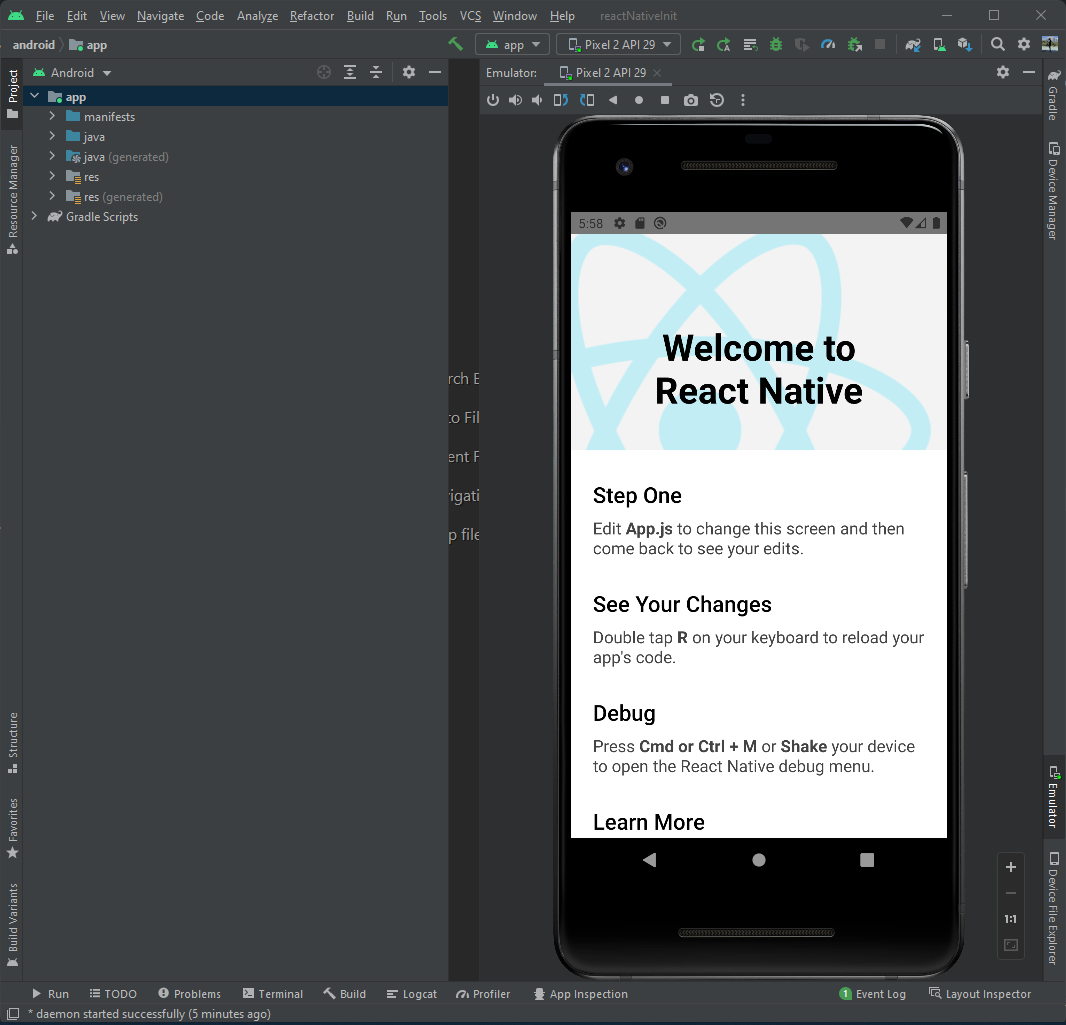
\includegraphics[width=0.8\textwidth]{Theorie/ReactNative/AndroidStudio.png}
    \caption{Die Beispiel-App in Android Studio}
  \end{center}
\end{figure}

  \item Mit einem physischen Android-Gerät:\\
Als erstes aktiviert man auf dem Gerät in den Einstellungen USB-Debugging und schließt es mittels
USB an den PC an. Wenn alle Treiber installiert sind, müsste es dann direkt in Android Studio
erkannt werden, um die App zu installieren.

Jetzt muss noch ein Tunnel über die USB-Verbindung erzeugt werden, damit das Gerät darüber mit dem
lokalen Metro-Server kommunizieren kann. Man listet alle Geräte auf und erzeugt dann mit der
Device-Identifikation einen Tunnel.

\begin{lstlisting}
C:\example\reactNativeInit> adb devices
List of devices attached
34299o5j85o496g3        device
emulator-8125           device

C:\example\reactNativeInit> adb -s 34299o5j85o496g3 reverse tcp:8081 tcp:8081
8081
\end{lstlisting}

\end{enumerate}
\newpage
\section{Expo CLI}
\label{expocli}
Die Entwickler von React Native selbst empfehlen allen Anfängern im Gebiet App-Entwicklung die
Verwendung der Expo CLI \cite{expocli}, welche eine vereinfachte Variante einer React Native Anwendung erzeugt.

Als Vorteil zählt auf jeden Fall die Geschwindigkeit, mit der eine neue App auf einem neuen Gerät
getestet werden kann. Dies ist meist innerhalb weniger Minuten möglich.

Ein wichtiger Nachteil ist jedoch, dass man in einem Expo-Projekt eingeschränkten Zugriff auf
Schnittstellen des Betriebssystems hat, es sind im Projekt nicht einmal die Ordner android und ios
vorhanden, um Änderungen vorzunehmen.

\subsection{Installation und Erstellung einer Expo App}
Um eine Expo React Native Anwendung erstellen zu können benötigt man als erstes \nameref{nodejs} und
den darin enthaltenen Node Package Manager. In einer Kommandozeile führt man nun folgende Befehle
aus, um die Expo-CLI im globalen Kontext zu installieren und anschließend ein Expo Projekt zu
erstellen. Nach der Auswahl für die Vorlage wird das Projekt erstellt.

\begin{lstlisting}
C:\example> npm install -g expo-cli
added 1549 packages, and audited 1550 packages in 1m

C:\example>expo init expoInitBlank
? Choose a template: - Use arrow-keys. Return to submit.
    ----- Managed workflow -----
>   blank               a minimal app as clean as an empty canvas
    blank (TypeScript)  same as blank but with TypeScript configuration
    tabs (TypeScript)   several example screens and tabs using react-navigation and TypeScript
    ----- Bare workflow -----
    minimal             bare and minimal, just the essentials to get you started
\end{lstlisting}

\begin{itemize}
\item Ordner:
  \begin{itemize}
  \item \textbf{.expo-shared, .git}:\\
  In den Ordnern .expo-shared, .git und .vscode befinden sich lediglich Konfigurationsdateien für
  Expo selbst und die Versionsverwaltungssoftware Git.

  \item \textbf{assets}:\\
  Der Ordner assets ist für das Abspeichern von statischen Ressourcen, wie Bilder, Icons oder
  ähnliches gedacht.
  \end{itemize}

\newpage

\item Dateien:
  \begin{itemize}
  \item \textbf{app.json}\\
  In app.json werden bei der Erstellung mit Expo zusätzliche Informationen zur App abgespeichert,
  darunter auch die Versionsnummer, Bildschirmausrichtung und noch viele weitere Optionen.

  \item \textbf{yarn.lock}\\
  Expo erzeugt ein Blank-Template standardmäßig mit Yarn, man kann aber auch stattdessen mit dem
  Tag -{}-npm bei der Projekterstellung NPM einbinden.
  \end{itemize}
\end{itemize}

Die App kann nun sofort getestet werden, als erstes startet man wieder den JavaScript-Bundler
\nameref{metrobundler} mit folgendem Befehl:

\begin{figure}[H]
  \begin{center}
    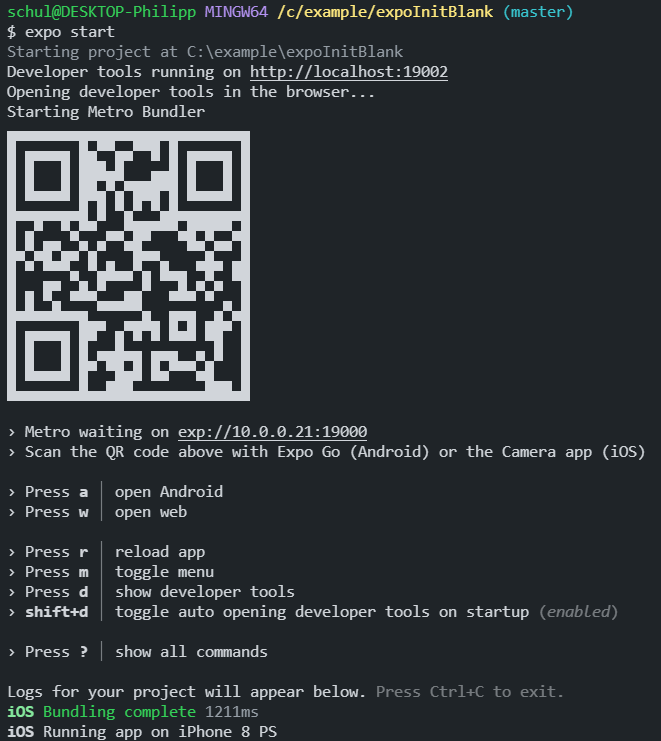
\includegraphics[width=0.6\textwidth]{Theorie/ReactNative/ExpoStart.png}
    \caption{Expo beim Start}
  \end{center}
\end{figure}

\begin{figure}[H]
  \begin{center}
    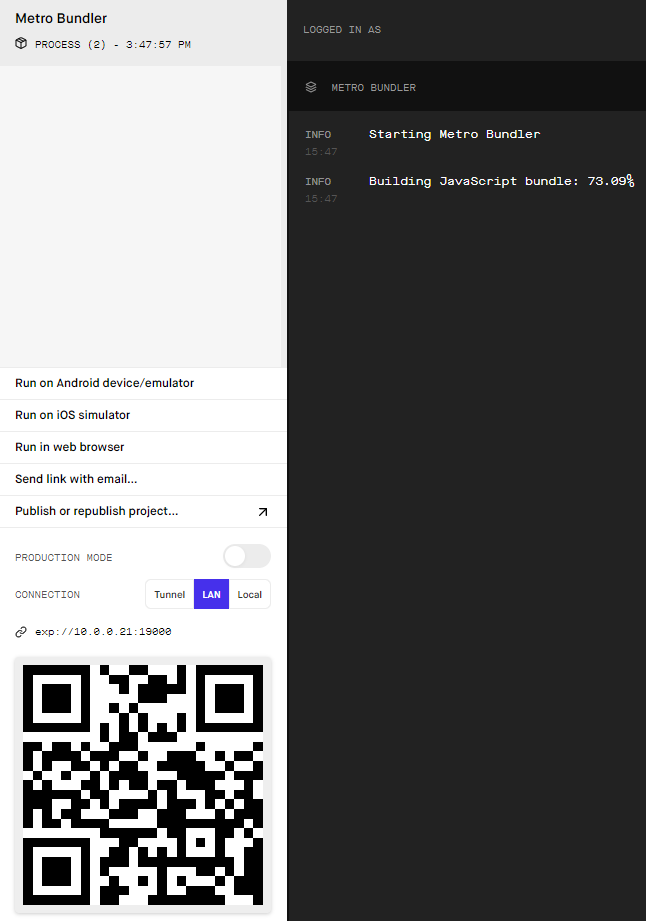
\includegraphics[width=0.6\textwidth]{Theorie/ReactNative/ExpoWebClient.png}
    \caption{Webinterface von Expo}
  \end{center}
\end{figure}

Nach dem Start wird im Webbrowser ein Entwickler-Menü geöffnet, auf dem noch einmal der QR-Code
und noch einige weitere hilfreiche Funktionen zu finden sind.

Um nun die App zu testen, muss man noch die ExpoGo App auf seinem Mobiltelefon installieren und den
gezeigten QR-Code scannen, während man im selben Netzwerk ist. Danach wird eine Bundle-Anfrage an
den lokalen Metro-Server geschickt, er kompiliert unser Projekt und schickt es an den Client.

\begin{figure}[H]
  \begin{center}
    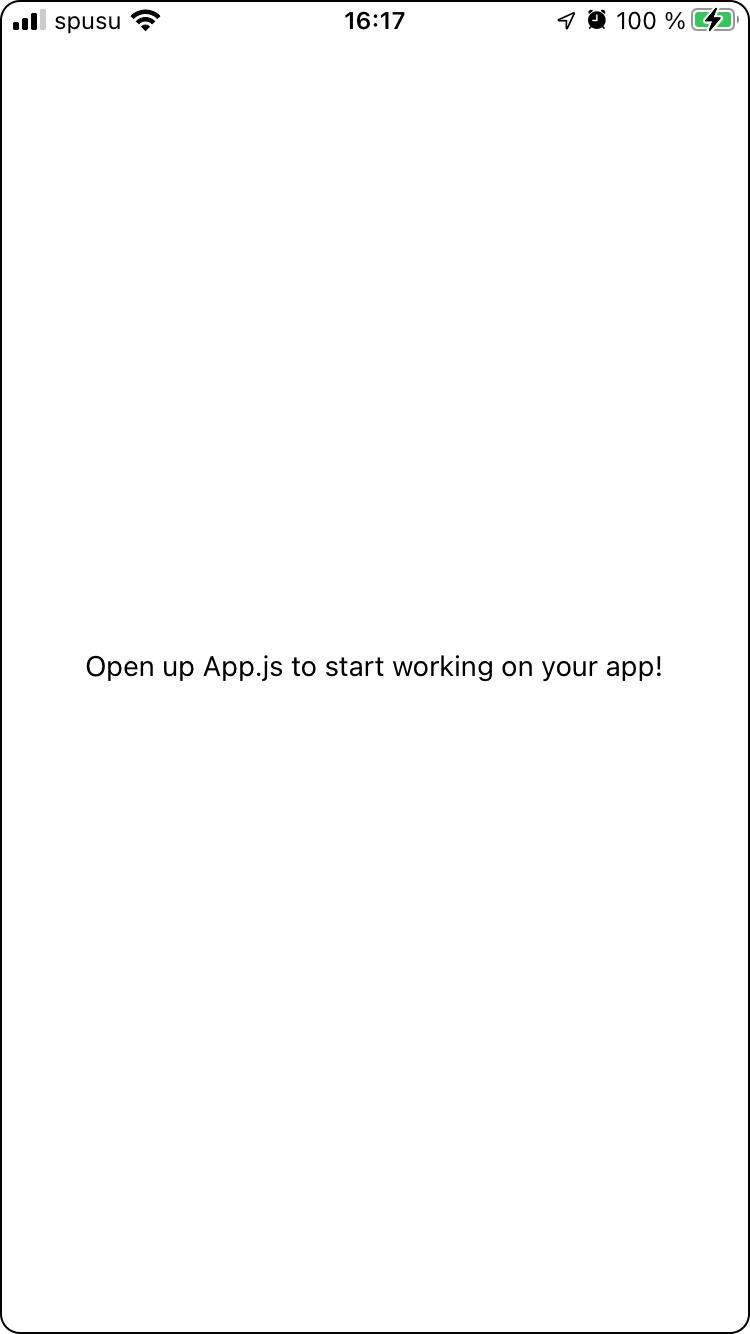
\includegraphics[width=0.5\textwidth]{Theorie/ReactNative/ExpoBlank.jpeg}
    \caption{Die weiße Leinwand von Expo}
  \end{center}
\end{figure}

\subsubsection{Expo Eject}
Wie bereits vorher schon erwähnt, hat es einige Nachteile seine App mit Expo zu machen. Um aber
einen schnellen Prototypen zu bauen ist das Framework perfekt. Um also eine Expo App in eine
vollwertige React Native Anwendung umzuwandeln, benötigt man folgenden Befehl.

\begin{lstlisting}
C:\example\expoInitBlank> expo eject
\end{lstlisting}

Man wird bei einer Eingabeaufforderung darüber informiert, dass dieser Prozess nicht rückgängig
gemacht werden kann.
\newpage

\section{Andere CLIs}
\begin{itemize}
  \item IgniteCLI \cite{ignitecli}
  \item Create-React-Native-App \cite{createReactNativeApp}
\end{itemize}